\documentclass[a4paper,10pt]{report}
\usepackage[utf8]{inputenc}
\usepackage{listings}
\usepackage{url}
\usepackage{subfigure}
\usepackage[pdftex]{graphicx}
\usepackage{wrapfig}

% Title Page
\title{}
\author{S. Koulouzis}


\begin{document}
\maketitle
\section{Mounting lobcder manually on Ubuntu, Debian linux.}


First of all, we need to install the davfs2 package. davfs2 provides the ability to access WebDAV resources like a typical filesystem, allowing for use by standard applications with no built-in support for WebDAV. 

\begin{lstlisting}
$sudo apt-get install davfs2
\end{lstlisting}


Next create, create the mount directory:

\begin{lstlisting}
$sudo mkdir /media/$USER/lobcder
\end{lstlisting}

Before mounting lobcder we need to obtain a ticket from \url{https://portal.vph-share.eu/} that we will use for authenticating our selfs with lobcder. Although we could use that ticket directly, davfs2 and most of WebDAV clients are unable to use passwords longer that 256 characters. To go around this we'll need to get a short translation of our ticket.

\begin{enumerate}
 \item Log in to \url{https://portal.vph-share.eu/}
 \item Go to \url{https://portal.vph-share.eu/profile/} and click ``Copy your Authentication Ticket to clipboard''
 \item Using a browser go to \url{https://lobcder.vph.cyfronet.pl/lobcder/urest/getshort/LONG\_TICKET} and we will get a short translation of our ticket . LONG\_TICKET is the ticket we copied form the previous step.
\end{enumerate}

Now we are ready to mount lobcder. 

\begin{lstlisting}
$sudo mount -t davfs https://lobcder.vph.cyfronet.pl/lobcder/dav \
/media/$USER/lobcder -o rw,uid=$USER
\end{lstlisting}

You will be asked for a username and a password. For the username use the one you used to log in to \url{https://portal.vph-share.eu/}. For a password use the short token that you got from \url{https://lobcder.vph.cyfronet.pl/lobcder/urest/getshort/LONG_TICKET}. 
Next we press 'y' to accept lobcder's certificate and lobcder is mounted on our machine. 

You can also put your username/password in /etc/davfs2/secrets

\begin{lstlisting}
$sudo echo "https://lobcder.vph.cyfronet.pl/lobcder/dav  username  password" >> /etc/davfs2/secrets
\end{lstlisting}


Note that with this method you will have to re-enter you short token after some days since it's designed to expire.  




\section{Using LOBCDER with cadaver}
For a quick access to lobcder we can also use cadaver. cadaver is a command-line WebDAV client for Unix. It supports file upload, download, on-screen display, namespace operations (move/copy), collection creation and deletion, and locking operations.

First of all, we need to install the cadaver package

\begin{lstlisting}
$sudo apt-get install cadaver
\end{lstlisting}



Before using cadaver we need to obtain a ticket from \url{https://portal.vph-share.eu/} that we will use for authenticating our selfs with lobcder. Although we could use that ticket directly, cadaver and most of WebDAV clients are unable to use passwords longer that 256 characters. To go around this we'll need to get a short translation of our ticket.


\begin{enumerate}
 \item Log in to \url{https://portal.vph-share.eu/}
 \item Go to \url{https://portal.vph-share.eu/profile/} and click ``Copy your Authentication Ticket to clipboard''
 \item Using a browser go to \url{https://lobcder.vph.cyfronet.pl/lobcder/urest/getshort/LONG\_TICKET} and we will get a short translation of our ticket . LONG\_TICKET is the ticket we copied form the previous step.
\end{enumerate}

Now we can log in with cadaver:

\begin{lstlisting}
$cadaver https://lobcder.vph.cyfronet.pl/lobcder/dav
\end{lstlisting}



You will be asked for a username and a password. For the username use the one you used to log in to \url{https://portal.vph-share.eu/}. For a password use the short token that you got from \url{https://lobcder.vph.cyfronet.pl/lobcder/urest/getshort/LONG_TICKET}. 



\section{Using LOBCDER Nautilus on Ubuntu}

For a GUI access to lobcder we can use Nautilus. Nautilus is the default file manager for Ubuntu. 

Before using cadaver we need to obtain a ticket from \url{https://portal.vph-share.eu/} that we will use for authenticating our selfs with lobcder. 


\begin{enumerate}
 \item Log in to \url{https://portal.vph-share.eu/}
 \item Go to \url{https://portal.vph-share.eu/profile/} and click ``Copy your Authentication Ticket to clipboard''
\end{enumerate}

\subsection{Ubuntu 12}

Click on the File Folder icon in the left launcher bar.

\begin{figure}
	\centering
	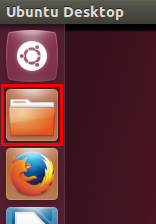
\includegraphics[width=0.3\textwidth]{graphics/ver12_1.png}\label{fig:ver12_1}
\end{figure}




Move your cursor to the top of the screen to reveal the File menu. Click on the File menu to open it, then select Connect to Server.

\begin{figure}
	\centering
	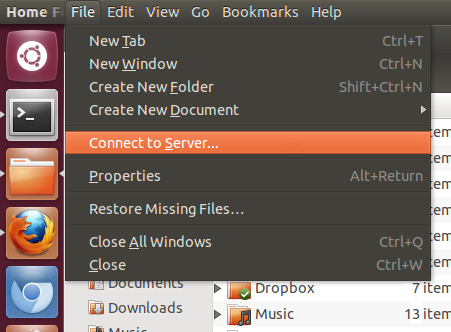
\includegraphics[width=0.3\textwidth]{graphics/ver12_2.png}\label{fig:ver12_2.png}
\end{figure}




In the Connect to Server window, enter the following:
\begin{itemize}
 \item Server: lobcder.vph.cyfronet.pl
 \item Port: 443
 \item Type: Secure WebDave (HTTPS)
 \item Folder: /lobcder/dav
 \item User name: Use the one you used to log in to \url{https://portal.vph-share.eu/}
 \item Password: paste the token you got from \url{https://portal.vph-share.eu/profile/}
\end{itemize}


Click Connect.

\subsection{Ubuntu 13-14}

Click on the File Cabinet icon in the left launcher bar.
\begin{figure}
	\centering
	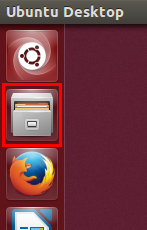
\includegraphics[width=0.3\textwidth]{graphics/ver13_1.png}\label{fig:ver13_1.png}
\end{figure}


In the left-hand navigation bar, select Connect to Server (located under Network.)


\begin{figure}
	\centering
	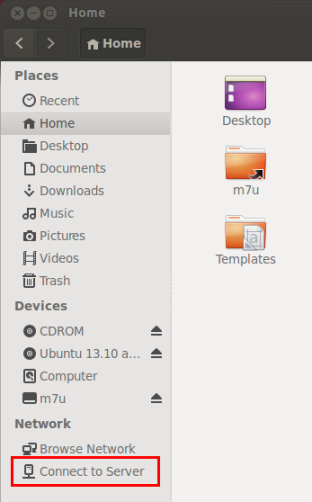
\includegraphics[width=0.3\textwidth]{graphics/ver13_2.png}\label{fig:ver13_2.png}
\end{figure}


In the Connect to Server window, enter the following URL into the Server Address field: \url{davs://lobcder.vph.cyfronet.pl/lobcder/dav}


\begin{figure}
	\centering
	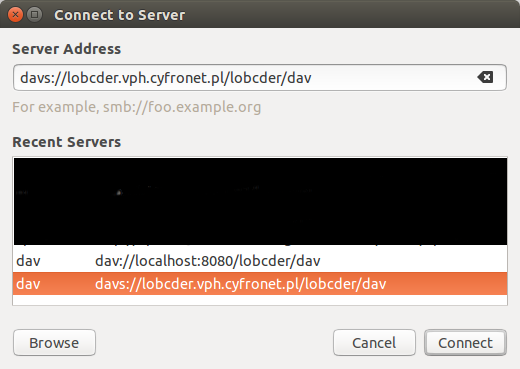
\includegraphics[width=0.3\textwidth]{graphics/ver13_3.png}\label{fig:ver13_3.png}
\end{figure}



You will be prompted for your username and password. For the username use the one you used to log in to \url{https://portal.vph-share.eu/}. For the password paste the token you got from \url{https://portal.vph-share.eu/profile/}

\begin{figure}
	\centering
	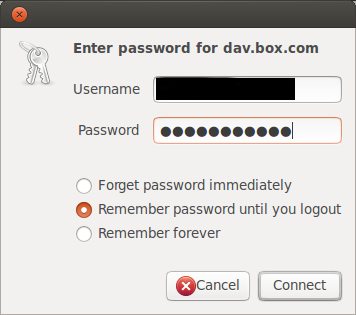
\includegraphics[width=0.3\textwidth]{graphics/ver13_4.png}\label{fig:ver13_4.png}
\end{figure}



\section{Upload data into LOBCDER using the Master Interface}


Log in to \url{https://portal.vph-share.eu/} 
In \url{https://portal.vph-share.eu/data/} click on ``Upload Data''
Click on ``FileStore Upload Unstructured Data (e.g. images and scans)''
Select on the folder you want to upload data to
On the top left corner click on ``upload'' 


\end{document}     
